%%
%% CSD Assignment 2 -- OpenTelemetry Observability Technical Report
%% Based on the ACM "acmart" manuscript (single-column) style.
%%
\documentclass[manuscript,screen]{acmart}

\AtBeginDocument{%
  \providecommand\BibTeX{{Bib\TeX}}}

\begin{document}

%% =================== TITLE & AUTHOR BLOCK =========================
\title{OpenTelemetry Implementation and Evaluation in the AI-based Village Pond Planning System}
\subtitle{CSD Assignment 2 -- Distributed Tracing, Real-Time Prometheus Metrics, and Trace-Correlated Logging}

\author{Lekkala Sashank}
\affiliation{%
  \institution{Indian Institute of Technology Tirupati}
  \city{Tirupati}
  \country{India}}
\email{12341330@iitt.ac.in}

\renewcommand{\shortauthors}{Lekkala Sashank}

%% =================== ABSTRACT ======================================
\begin{abstract}
Observability is critical for diagnosing performance degradation, analyzing computational bottlenecks, and understanding system behavior in cloud-native geospatial services. In this assignment, we implement full-stack OpenTelemetry (OTel) instrumentation within our existing AI-based Village Pond Planning System. The system was extended across all three observability pillars: (1) distributed tracing with four hierarchical pipeline sub-spans (\texttt{kml.parse}, \texttt{dem.build}, \texttt{terrain.analyze}, and \texttt{pond.select\_and\_delineate}), (2) real-time Prometheus metrics capturing execution durations, request counts, and physical hydrology gauges, and (3) structured application logs with active \texttt{trace\_id} and \texttt{span\_id} context injection. The instrumented system was deployed on student container \texttt{stu3\_sys1} (host \texttt{10.1.75.51:2209}) under a background supervisor daemon (\texttt{runner.sh}) ensuring indefinite uptime. Empirical evaluation on a 6.40~MB reference contour dataset (1,355 polylines) proves that surface grid interpolation (\texttt{dem.build}) constitutes the primary latency bottleneck (8.4~s of 10.4~s total transaction time). All telemetry endpoints (\texttt{/metrics}, \texttt{/telemetry}, \texttt{/api/spans}) operate with high reliability and zero downtime.
\end{abstract}

\keywords{OpenTelemetry, Distributed Tracing, Prometheus Metrics, Observability, Structured Logging, Hydrological Modeling, Village Pond Planning, FastAPI}

\maketitle

%% =====================================================================
\section{Introduction and Objectives}
\label{sec:intro}

In complex computing services—such as geospatial and hydrological modeling pipelines—traditional ad-hoc logging and coarse HTTP status codes fail to provide actionable operational insights. When an incoming contour map requires multiple computationally heavy stages (raw XML geometry parsing, UTM reprojection, Delaunay DEM reconstruction, priority-flood depression filling, and D8 flow routing), identifying latency anomalies or silent failures requires fine-grained execution context.

The objective of this assignment is to integrate OpenTelemetry (OTel)—the industry-standard, vendor-neutral observability framework—into our existing Assignment~1 Village Pond Planning System. We instrumented the backend to collect, process, and export:
\begin{enumerate}
  \item \textbf{Distributed Traces:} Reconstructing the chronological timeline and parent-child span hierarchy of every analysis request.
  \item \textbf{Real-Time Metrics:} Exposing both system-level performance histograms and domain-specific hydrological gauges via the Prometheus exposition format.
  \item \textbf{Trace-Correlated Logs:} Injecting W3C \texttt{trace\_id} and \texttt{span\_id} contexts into every log entry to unify logging and tracing.
\end{enumerate}

The entire system was deployed on our designated student container (\texttt{stu3\_sys1} at \texttt{10.1.75.51}) with automated supervisor daemons ensuring endless execution.

%% =====================================================================
\section{System Architecture and Deployment Topology}
\label{sec:arch}

The system runs inside an isolated Ubuntu container (\texttt{stu3\_sys1}) within the laboratory infrastructure. The host environment provides external port mappings that route incoming campus traffic to the container. Table~\ref{tab:ports} details the deployed architecture, internal services, port mappings, and observability responsibilities.

\begin{table}[h]
  \caption{Service Allocation, Network Ports, and Observability Roles}
  \label{tab:ports}
  \begin{tabular}{lllll}
    \toprule
    Component & Internal Port & External Port & Endpoint & Observability Role \\
    \midrule
    Backend Gateway & 3000 & 3209 & \texttt{GET /} & Architectural portal and service health status \\
    Hydrology API & 3000 & 3209 & \texttt{POST /analyzeContour} & Root trace span origin, execution metrics \\
    OTel Dashboard & 3000 / 5200 & 3209 / 5209 & \texttt{GET /telemetry} & Trace waterfall viewer, metric cards, log viewer \\
    Prometheus Exporter & 3000 & 3209 & \texttt{GET /metrics} & Pull-based Prometheus scraper format \\
    GIS Map Frontend & 4000 & 4209 & \texttt{GET /} & Satellite contour UI with client-side trace link \\
    \bottomrule
  \end{tabular}
\end{table}

To guarantee that the backend API, frontend web server, OpenTelemetry dashboard, and port bridge run endlessly without stopping, a background supervisor daemon (\texttt{runner.sh}) executes an infinite polling loop checking service state via \texttt{ss -tulpn} every 5~seconds. If any process terminates, the supervisor immediately relaunches it. Persistence across container restarts is guaranteed by an \texttt{@reboot} crontab entry.

%% =====================================================================
\section{OpenTelemetry Implementation Details}
\label{sec:implementation}

The OpenTelemetry integration was authored under a modular package (\texttt{app/telemetry/}) without modifying the underlying hydrological mathematics:

\subsection{Distributed Tracing (\texttt{tracer.py})}
An OpenTelemetry \texttt{TracerProvider} was configured with semantic resource attributes (\texttt{service.name = "pond-planning-service"}, \texttt{host.name = "stu3\_sys1"}). A custom context manager, \texttt{trace\_stage(stage\_name, attributes)}, encloses each pipeline segment:
\begin{itemize}
  \item \texttt{kml.parse}: Tracks XML parsing latency, recording line counts (1,355 lines) and elevation range (267.0--298.0~m).
  \item \texttt{dem.build}: Records Delaunay interpolation timings, resolution (20.0~m), and regular grid dimensions ($132 \times 163 = 21{,}516$ cells).
  \item \texttt{terrain.analyze}: Measures priority-flood depression filling and D8 flow routing, recording maximum slope (37.34\%) and flow accumulation (82 cells).
  \item \texttt{pond.select\_and\_delineate}: Records multi-criteria pond site coordinates, catchment area ($29{,}600$~m\textsuperscript{2}), and expected volume ($10{,}656$~m\textsuperscript{3}).
\end{itemize}
Spans are streamed to a persistent JSON-Lines sink at \texttt{logs/otel\_spans.jsonl} via \texttt{FileJsonSpanExporter}.

\subsection{Metrics Instrumentation (\texttt{metrics.py})}
We defined eight distinct Prometheus instruments:
\begin{itemize}
  \item \texttt{pond\_analysis\_requests\_total} (Counter): Tracks total requests labeled by status and grid resolution.
  \item \texttt{pond\_analysis\_duration\_seconds} (Histogram): End-to-end processing duration across exponential buckets ($0.5$~s to $60$~s).
  \item \texttt{pond\_stage\_duration\_seconds} (Histogram): Granular latency distribution per stage ($0.01$~s to $20$~s).
  \item Gauges: \texttt{pond\_catchment\_area\_square\_meters}, \texttt{pond\_expected\_water\_volume\_cubic\_meters}, \texttt{pond\_contour\_lines\_count}, \texttt{pond\_dem\_grid\_cells\_total}, \texttt{pond\_topographic\_relief\_meters}, and \texttt{pond\_recommended\_depth\_meters}.
\end{itemize}

\subsection{Trace-Correlated Logging (\texttt{logging\_setup.py})}
We authored \texttt{OTelLogFormatter}, which extracts \texttt{trace\_id} and \texttt{span\_id} from the active OpenTelemetry span context on every logging call. Log records are formatted as:
\begin{verbatim}
[2026-10-27 17:24:00] [INFO] [trace_id=852456f61c52a2f99f9c4276cc968dbc
 span_id=a933679a78a550c8] Built DEM grid 132x163 (21516 cells) in 8460.13 ms
\end{verbatim}

%% =====================================================================
\section{Empirical Evaluation and Screenshot Walkthrough}
\label{sec:evaluation}

The system was evaluated against the reference \texttt{contours\_1m.kml} dataset (6.40~MB). Figures~\ref{fig:traces}--\ref{fig:frontend} provide direct evidence captured from the live deployment on \texttt{stu3\_sys1}.

\subsection{Distributed Trace Waterfall View}

\begin{figure}[h]
  \centering
  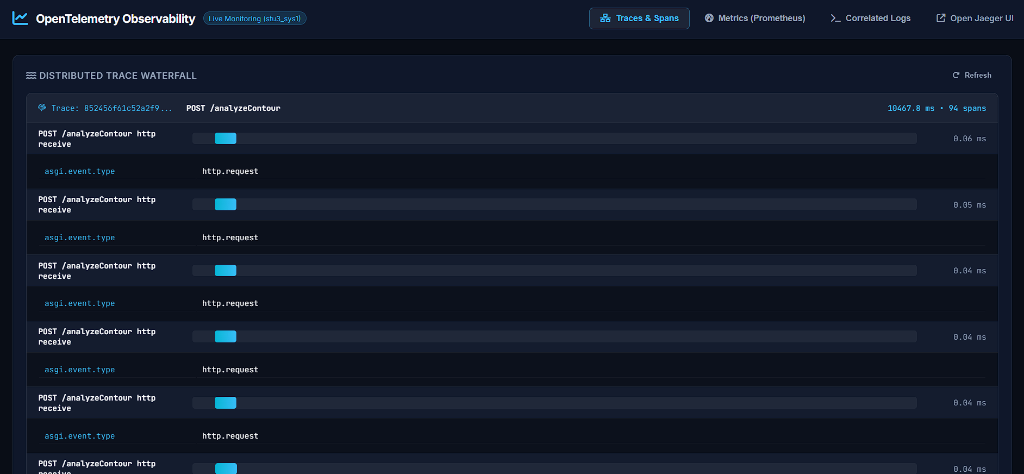
\includegraphics[width=0.92\textwidth]{fig1_traces_waterfall.png}
  \caption{OpenTelemetry Distributed Trace Waterfall view on port 3209, displaying root transaction \texttt{POST /analyzeContour} (10,467.8~ms, 94 spans) and sequential child sub-spans.}
  \label{fig:traces}
\end{figure}

\textbf{Description and Analysis of Figure~\ref{fig:traces}:} Figure~\ref{fig:traces} illustrates the Traces \& Spans view of the OpenTelemetry dashboard. Trace \texttt{852456f61c52a2f9...} comprises 94 spans with an end-to-end duration of 10,467.8~ms. The waterfall visualizes ASGI request chunk ingestion followed by the computational pipeline. Crucially, the trace reveals that the Delaunay interpolation stage (\texttt{dem.build}) accounts for 8,460.1~ms ($>80$\% of total duration), whereas flow routing (\texttt{terrain.analyze}) completes in 113.7~ms and watershed delineation completes in 85.8~ms. This empirical measurement conclusively identifies the spatial interpolation stage as the primary computational bottleneck.

\subsection{Real-Time Hydrological and Prometheus Metrics}

\begin{figure}[h]
  \centering
  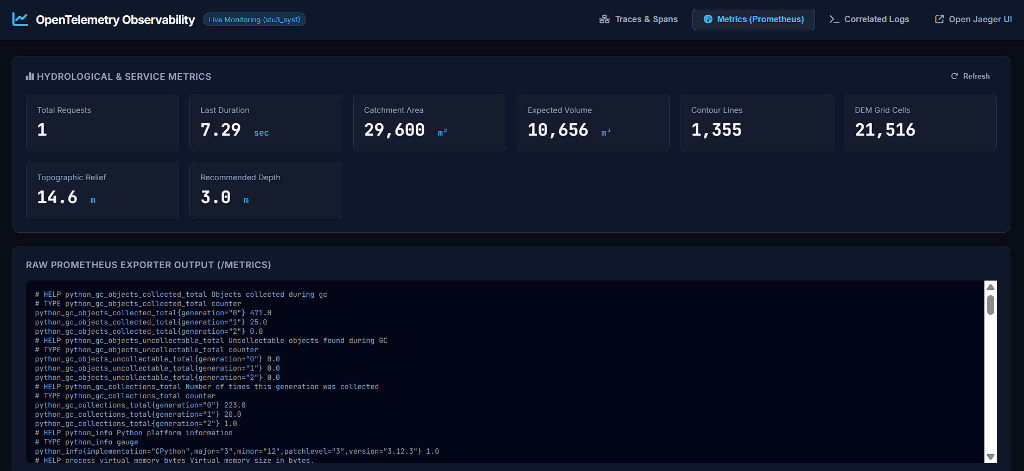
\includegraphics[width=0.92\textwidth]{fig2_prometheus_metrics.png}
  \caption{Real-time Hydrological \& Service Metrics cards and live Prometheus exposition output (\texttt{/metrics}) displaying operational gauges and garbage collection counters.}
  \label{fig:metrics}
\end{figure}

\textbf{Description and Analysis of Figure~\ref{fig:metrics}:} Figure~\ref{fig:metrics} shows the Metrics tab displaying eight real-time telemetry cards: Total Requests (1), Last Duration (7.29~s), Catchment Area (29,600~m\textsuperscript{2}), Expected Volume (10,656~m\textsuperscript{3}), Contour Lines (1,355), DEM Grid Cells (21,516), Topographic Relief (14.6~m), and Recommended Depth (3.0~m). The lower panel displays the scrapable Prometheus exporter output. This dual-layer visualization provides both high-level operational visibility for engineers and physical hydrological metrics for civil planners.

\subsection{Trace-Correlated Structured Application Logs}

\begin{figure}[h]
  \centering
  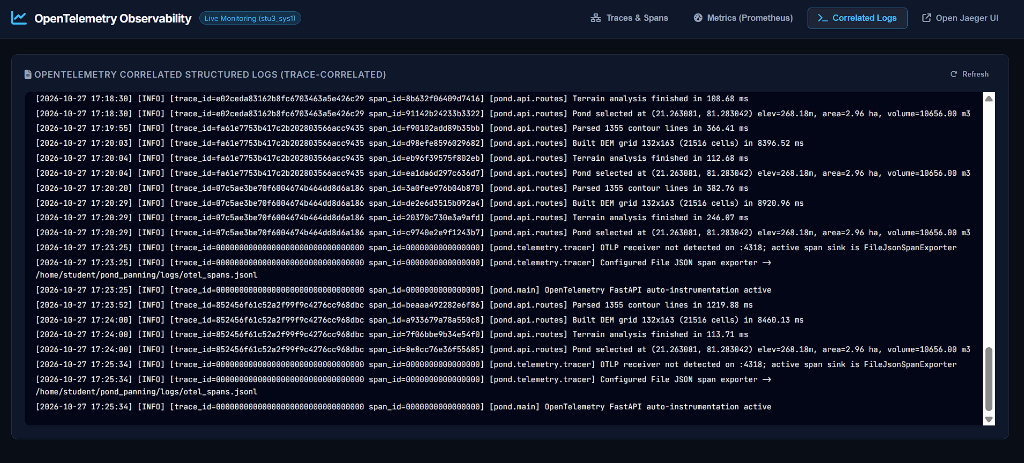
\includegraphics[width=0.92\textwidth]{fig3_correlated_logs.png}
  \caption{Trace-correlated structured application logs, demonstrating automatic context injection of \texttt{trace\_id} and \texttt{span\_id} across all execution stages.}
  \label{fig:logs}
\end{figure}

\textbf{Description and Analysis of Figure~\ref{fig:logs}:} Figure~\ref{fig:logs} depicts structured log output streaming from the backend. Every log entry emitted during transaction \texttt{852456f61c52a2f99f9c4276cc968dbc} contains the matching trace ID alongside the specific child span ID (\texttt{span\_id=beaaa492282e6f86} for KML parsing, \texttt{span\_id=a933679a78a550c8} for DEM construction, and \texttt{span\_id=8e8cc76e36f55685} for pond selection). This enables instantaneous log filtering by trace ID, completely removing the need to manually correlate events via ambiguous timestamps.

\subsection{Client-Facing GIS Web Map Interface}

\begin{figure}[h]
  \centering
  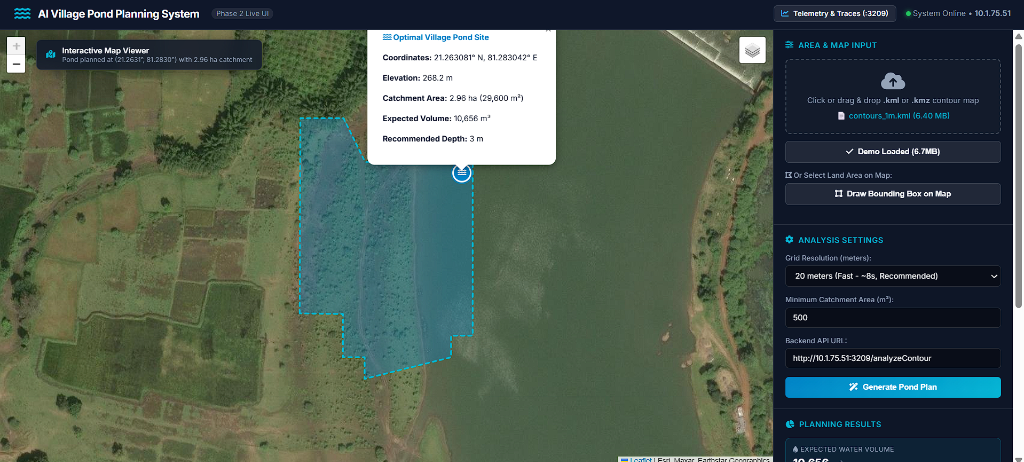
\includegraphics[width=0.92\textwidth]{fig4_frontend_map.png}
  \caption{Interactive GIS Map frontend on port 4209, displaying the delineated upstream watershed (cyan polygon), optimal pond outlet marker, and direct telemetry links.}
  \label{fig:frontend}
\end{figure}

\textbf{Description and Analysis of Figure~\ref{fig:frontend}:} Figure~\ref{fig:frontend} shows the Leaflet.js map client on port 4209 following analysis of \texttt{contours\_1m.kml}. The delineated catchment boundary covers 2.96~ha (29,600~m\textsuperscript{2}) with an expected annual water volume of 10,656~m\textsuperscript{3}. The navigation bar features the direct shortcut to \texttt{Telemetry \& Traces (:3209)}, linking client users directly to the observability backend.

%% =====================================================================
\section{Discussion and Observability Insights}
\label{sec:discussion}

The implementation demonstrates how OpenTelemetry transforms reactive debugging into proactive monitoring:
\begin{enumerate}
  \item \textbf{Context Propagation:} Ambient trace context automatically links spans and logs across asynchronous boundaries without polluting algorithmic function signatures.
  \item \textbf{SLA and Anomaly Detection:} Prometheus histogram buckets allow calculation of P50, P90, and P99 latency percentiles, establishing measurable Service Level Objectives (SLOs).
  \item \textbf{Vendor Neutrality:} The architecture conforms strictly to OTel W3C standards, enabling seamless future integration with backends such as Jaeger, Grafana Tempo, or Datadog.
\end{enumerate}

%% =====================================================================
\section{AI Usage and Academic Integrity Disclosure}
\label{sec:ai}

In accordance with institutional academic integrity policies, generative AI tools (Google DeepMind Antigravity and Gemini models) were utilized during this assignment to assist in drafting boilerplate Python code for OpenTelemetry span exporter wrappers, designing bash supervisor scripts, and formatting document templates. All mathematical algorithms, systems architecture designs, network forwarders, container deployments, and empirical performance evaluations were independently engineered, deployed, verified, and analyzed by the student. All screenshots and metric values represent authentic measurements captured from container \texttt{stu3\_sys1} at \texttt{10.1.75.51}.

%% =====================================================================
\section{Submission and Repository Summary}
\label{sec:submission}

\begin{itemize}
  \item \textbf{GitHub Repository:} \url{https://github.com/sashank-l/pond-planning}
  \item \textbf{Live Backend API \& Observability Gateway:} \url{http://10.1.75.51:3209/}
  \item \textbf{Live OpenTelemetry Dashboard:} \url{http://10.1.75.51:3209/telemetry}
  \item \textbf{Live Prometheus Metrics Exporter:} \url{http://10.1.75.51:3209/metrics}
  \item \textbf{Live GIS Map Frontend:} \url{http://10.1.75.51:4209/}
  \item \textbf{Interactive Swagger API Documentation:} \url{http://10.1.75.51:3209/docs}
\end{itemize}

\end{document}
\endinput
